%PROPERTY OF K.L.A.C.LAKSHAN lakshanklac@gmail.com
\documentclass[a4paper]{article}
\usepackage{graphicx}
\usepackage{amssymb}
\usepackage[a4paper,left=1 in,right=1  in,top=1 in,bottom=1 in]{geometry}
\usepackage{scrextend}
\usepackage{amsmath}
\usepackage{array}
\usepackage{lettrine}
\usepackage{caption}
\usepackage{tikz}
\usepackage{longtable}
\usepackage{comment}
\usetikzlibrary{calc}
\usepackage{booktabs}
\usepackage{indentfirst}
\usepackage{setspace}
\usepackage{hyperref}

\usepackage{titlesec}
%\titleformat{\section}{\normalfont\Large\bfseries\MakeUppercase}{}{0pt}{}


\captionsetup[table]{skip=0pt,singlelinecheck=on}

%function to stirke out rows in a table
\usepackage{tikz}
\newcommand{\pmark}[1]{\begin{tikzpicture}[overlay,remember picture]\node(#1)at (-.5em,.7ex){};\end{tikzpicture}}
\newcommand{\smark}[1]{\begin{tikzpicture}[overlay,remember picture]\draw(#1)--(+2.65,.7ex);\end{tikzpicture}}

%function for vspace
\newenvironment{conditions}
  {\par\vspace{\abovedisplayskip}\noindent\centering\begin{tabular}{>{$}l<{$} @{${}={}$} l}}
  {\end{tabular}\par\vspace{\belowdisplayskip}}
 
%function to change the fonstsize use \myfontsize command
%\newcommand\myfontsize{\fontsize{60pt}{18pt}\selectfont}

%\newcommand\HRule{\rule{\textwidth}{1pt}}


%------------------------------Doc Begins-----------------------------------------------------------------------------------------
\begin{document}

%------------------------------Cover-----------------------------------------------------------------------------------------
\begin{titlepage}

%BORDER
%\begin{tikzpicture}[remember picture, overlay]
%  \draw[line width = 2pt] ($(current page.north west) + (1 in,-1in)$) rectangle ($(current page.south east) + (-1in,1in)$);
%\end{tikzpicture}



% Syntax: \begin{addmargin}[<left indentation>]{<indentation>}
\begin{addmargin}[1em]{1em}
\begin{center}
% Upper part of the page
\begin{flushleft}
%{ }\\[7cm]
\end{flushleft}

% Title
\vspace{5cm} 
\textbf{\Huge PROGRAMME TO DETERMINE}\\[0.3cm]
\textbf{\Huge THE CRYSTAL STRUCTURE}\\[1cm]
\textbf{\Large Data Reduction of Diffractometer Experiment}\\[15cm]

\begin{minipage}{0.8\textwidth}
\begin{flushright} \large
\begin{tabular}{@{}l@{}}
K.L.A.C. LAKSHAN \\
\end{tabular}
\end{flushright}
\end{minipage}
\end{center}
\end{addmargin}
\end{titlepage}



%------------------------------Contents-----------------------------------------------------------------------------------------


\newpage

\tableofcontents
\newpage

%------------------------------Introduction----------------------------------------------------------------------------------------
\section{\underline{Introduction}}
\vspace{1em}
\lettrine{T}{} his is a programm written in order to determine the cystal structure after getting the data from a relavent experiment. 
Along with the structure, other informations like the lattice constant, atomic radius, denisity can be calculated.

The entire programme is written in Java.
 

\begin{figure}[h!]
\centering
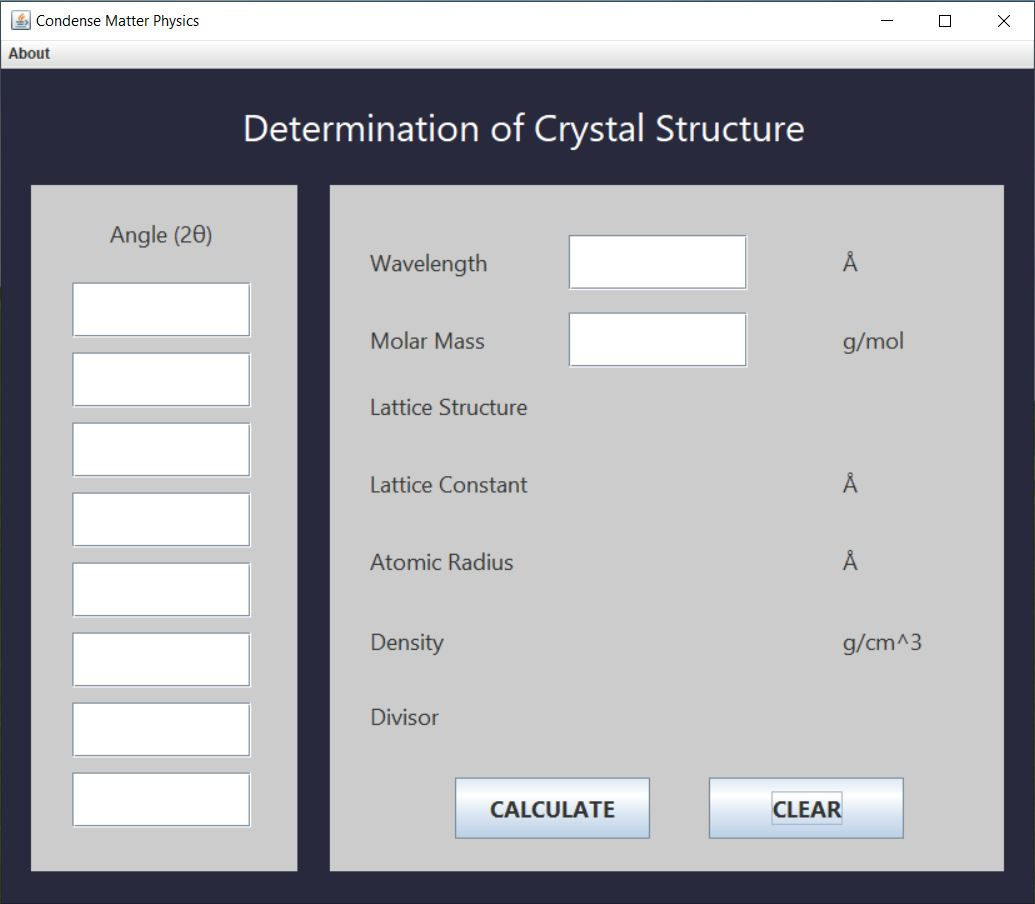
\includegraphics[width=402 px,height=307.625 px]{1}
\caption{User Interface}
\end{figure}


\newpage

%------------------------------Apparatus-----------------------------------------------------------------------------------------
\section{\underline{Interface}}
\vspace{1em}

\begin{figure}[h!]
\centering
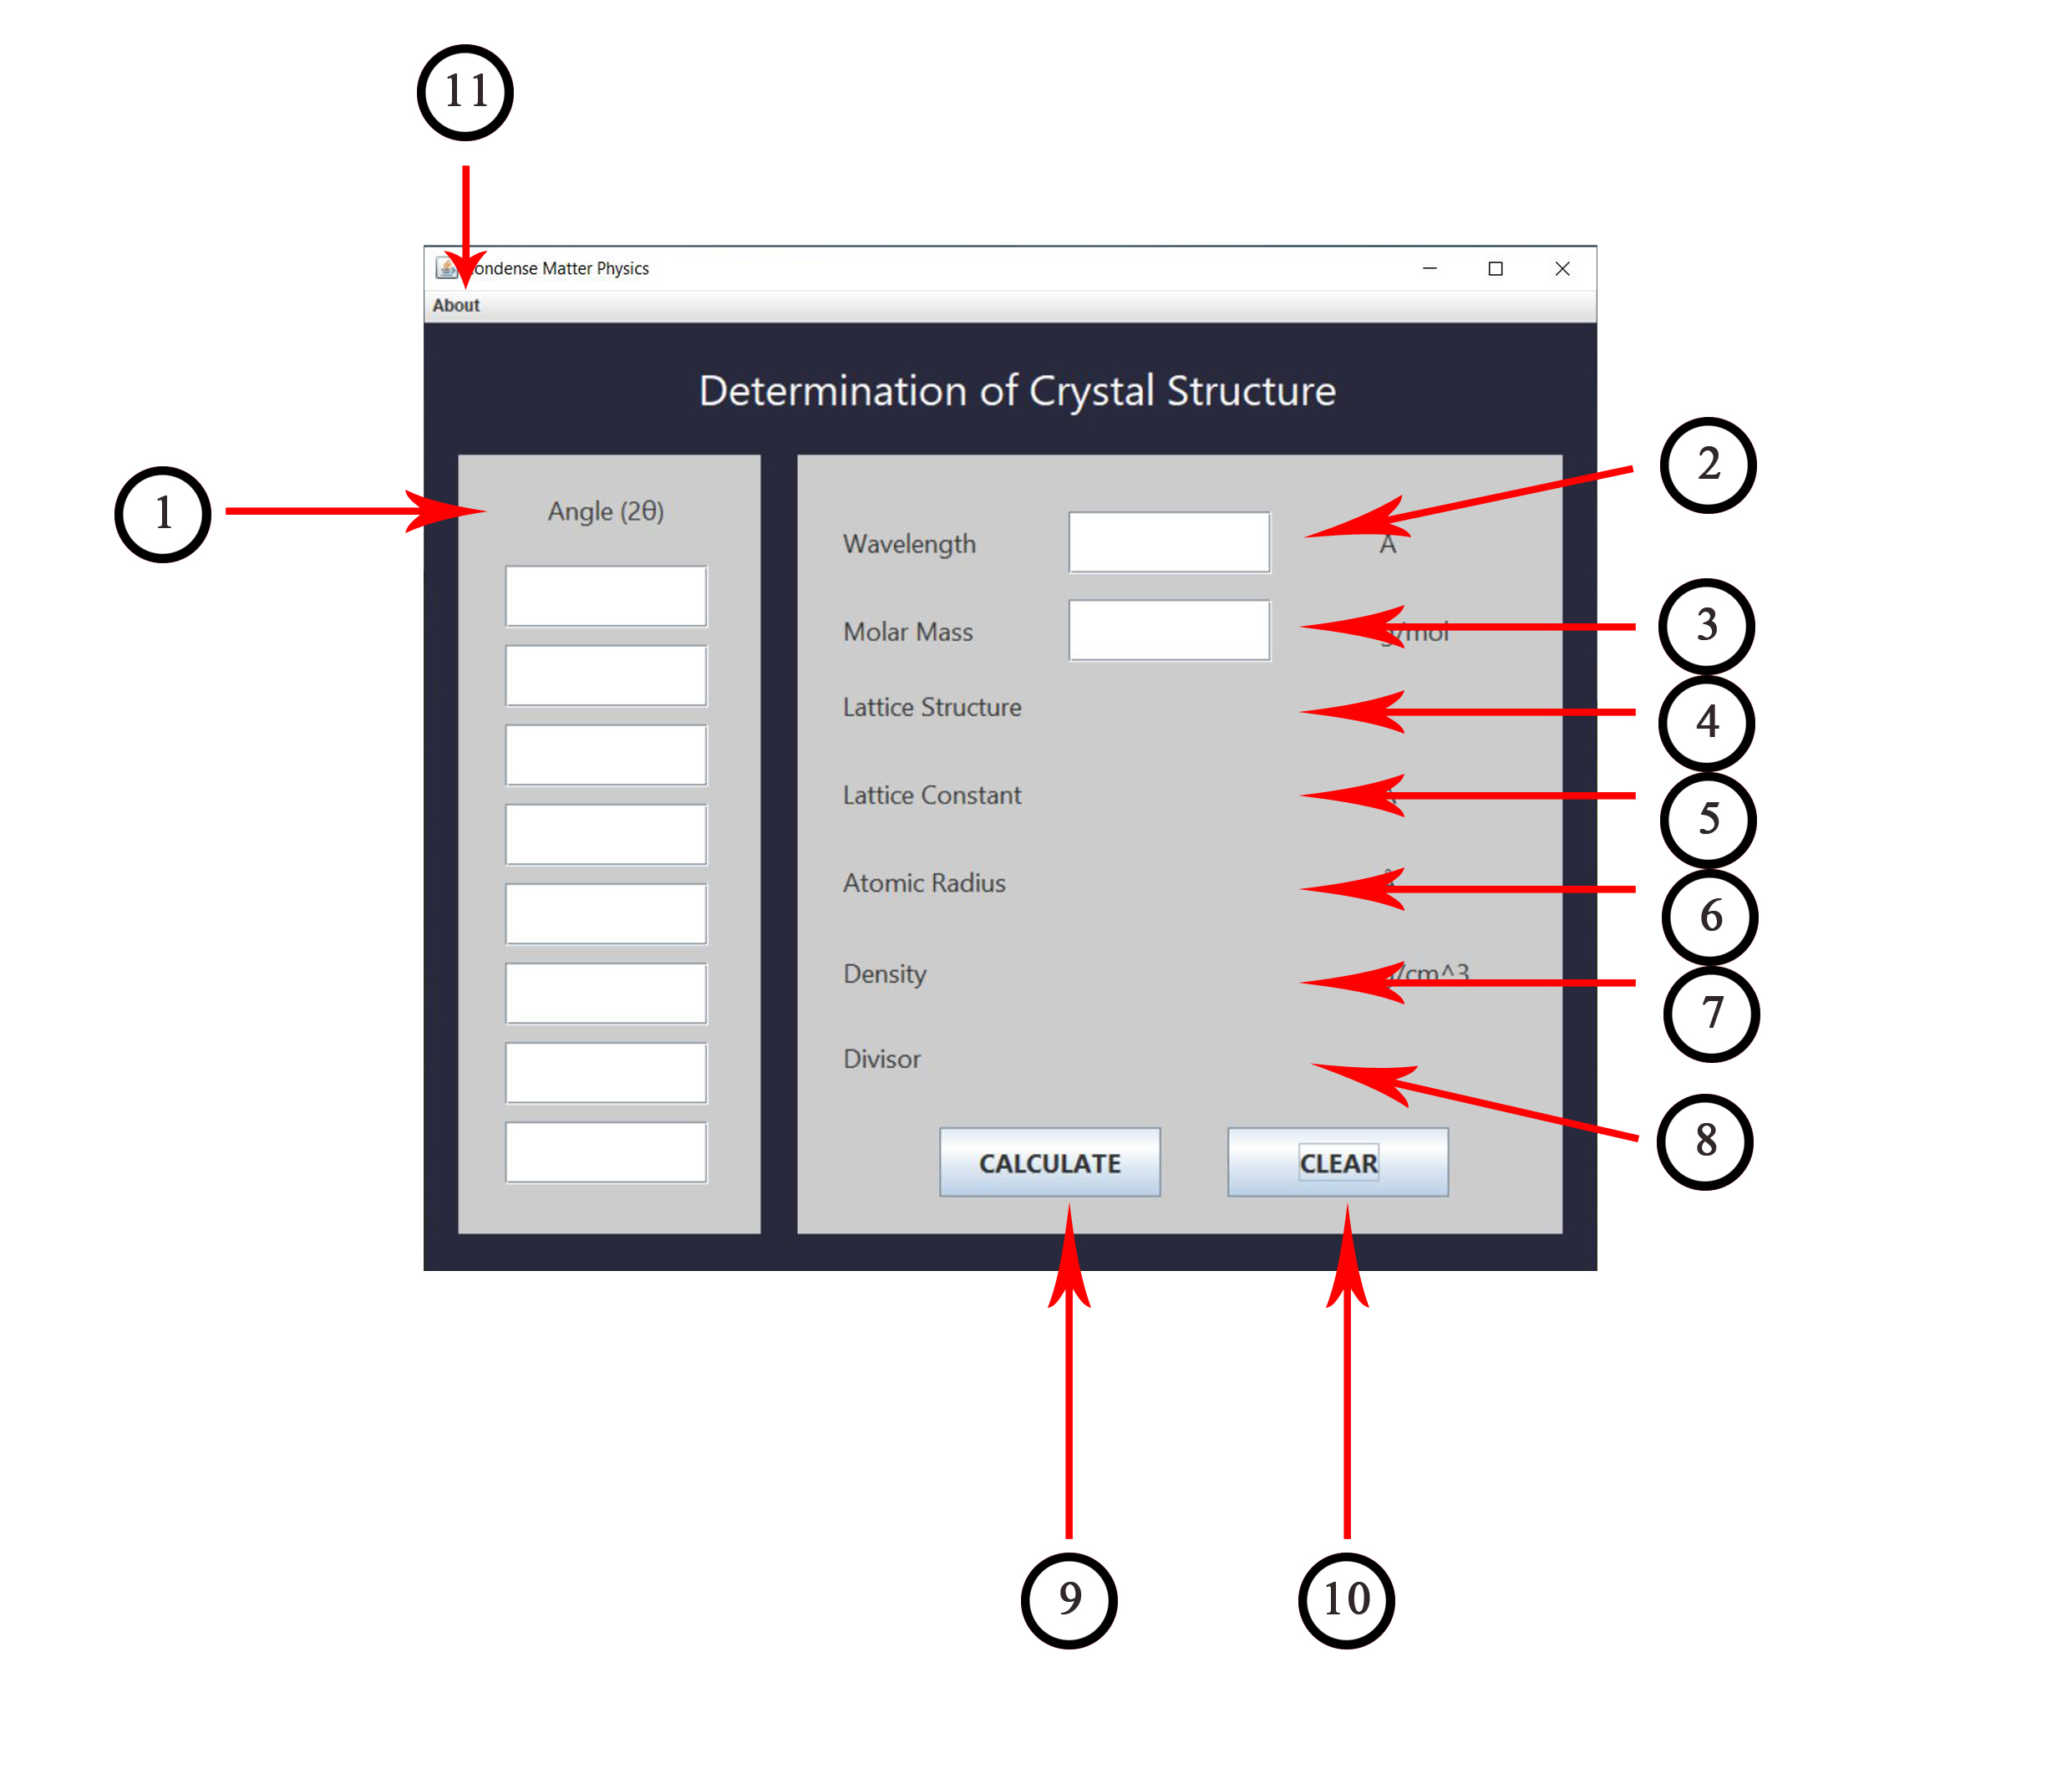
\includegraphics[width=402 px,height=307.625 px]{1.1}
\caption{Parts of the interface}
\end{figure}

\begin{enumerate}
\item[1.] Textfields to enter the angles.
\item[2.] Textfield to enter the value of wavelength used in the experiment.
\item[3.] Textfield to enter the molar mass of the crystal.
\item[4.] Display the lattice structure.
\item[5.] Display the lattice constant.
\item[6.] Display the atomic radius.
\item[7.] Display the density of the crystal.
\item[8.] Display the number which the sine squared value should divide if this is done manually.
\item[9.] Carry on the calculations ones clicked.
\item[10.] Clear all the textfields and results.
\item[11.] Display about the programme.
\end{enumerate}



%------------------------------Theory-----------------------------------------------------------------------------------------


\newpage
\section{\underline{Demonstration}}
\vspace{1em}
\begin{enumerate}
	\item[•] Case 1:
\end{enumerate}

Consider the angles 38.40, 44.50, 64.85, 77.90, 81.85, 98.40, 111.20 and wavelength 1.5418$\mathring{\mathrm{A}}$. Molar mass is given 66.6 $g mol^{-1}$ \footnote{\href{https://ocw.mit.edu/courses/3-091sc-introduction-to-solid-state-chemistry-fall-2010/ec60f89132400083b748c3dcde9e6e67_MIT3_091SCF09_hw18_sol.pdf}{MIT OCW}}
\\\\
\begin{figure}[h!]
\centering
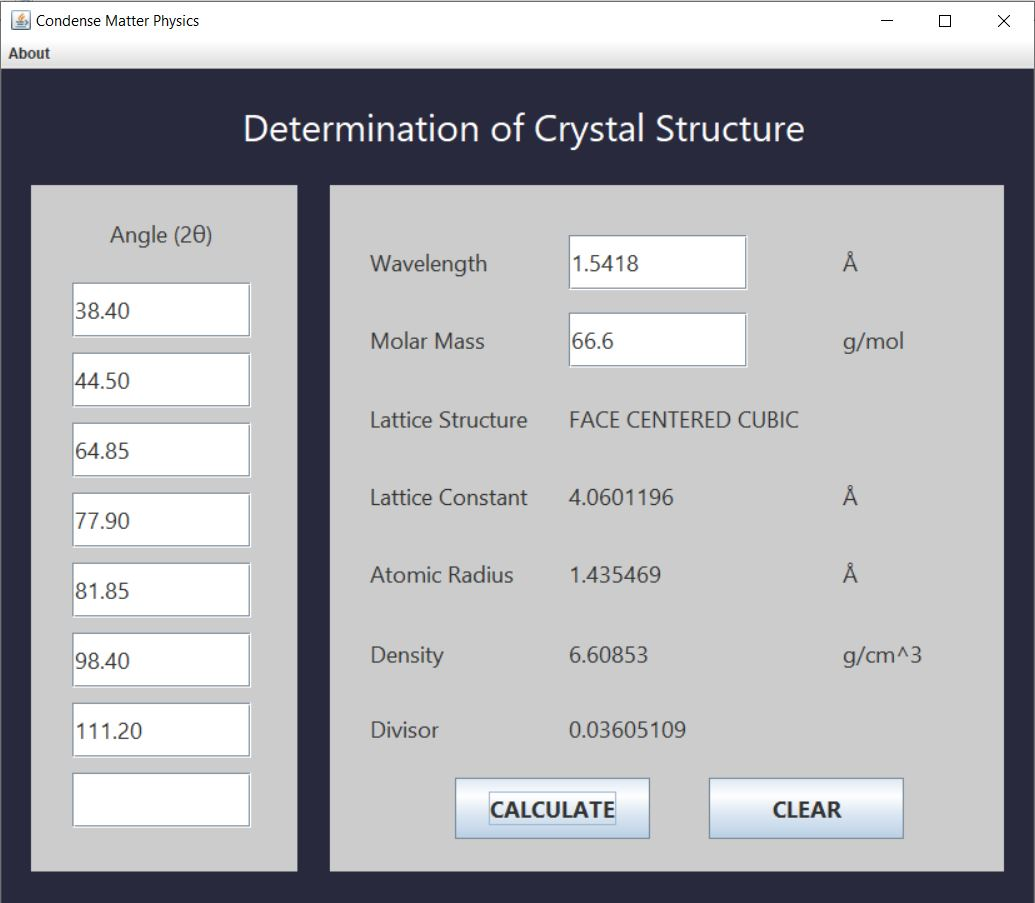
\includegraphics[width=402 px,height=307.625 px]{3.1}
\caption{Results for case 1}
\end{figure}

\newpage
\begin{figure}[h!]
\centering
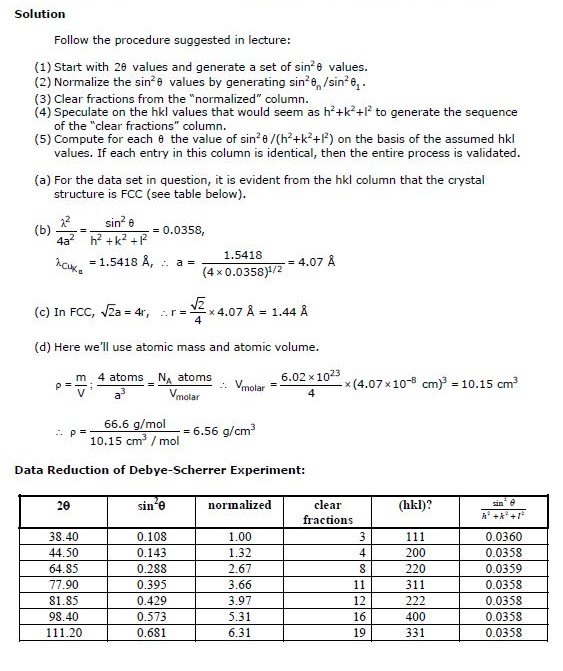
\includegraphics[width=450.4 px,height=536.8 px]{3}
\caption{Manually worked out solutions for case 1}
\end{figure}

This tally with the results of the programme.

\newpage

\begin{enumerate}
	\item[•] Case 2:
\end{enumerate}
Consider the angles 14.10, 19.98, 24.57, 28.41, 31.85, 34.98, 37.89, 40.61 and wavelength 0.574$\mathring{\mathrm{A}}$.  \footnote{\href{https://ocw.mit.edu/courses/3-091sc-introduction-to-solid-state-chemistry-fall-2010/ec60f89132400083b748c3dcde9e6e67_MIT3_091SCF09_hw18_sol.pdf}{MIT OCW}}
\\\\
\begin{figure}[h!]
\centering
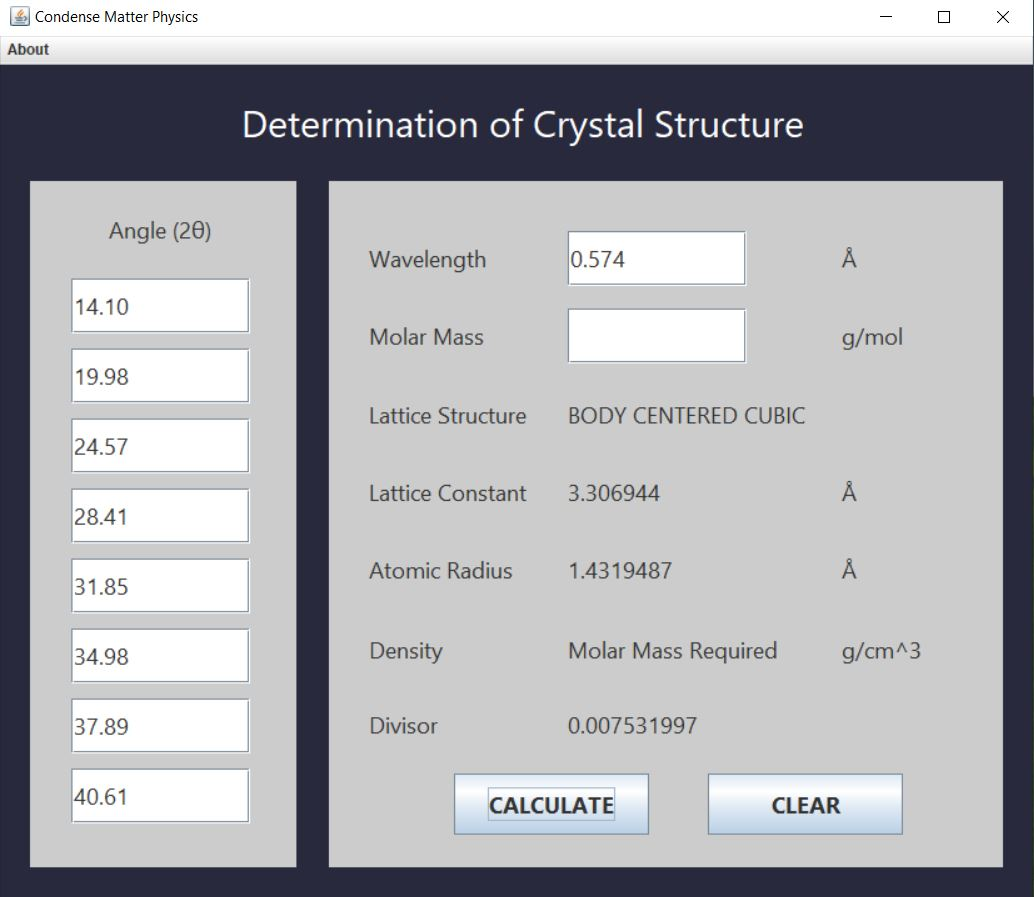
\includegraphics[width=402 px,height=307.625 px]{5}
\caption{Results for case 2}
\end{figure}

\newpage
\begin{figure}[h!]
\centering
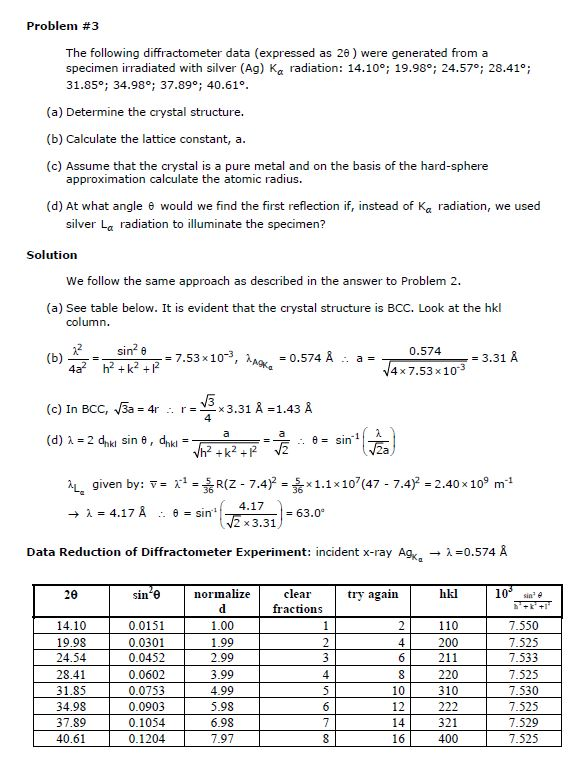
\includegraphics[width=450.4 px,height=536.8 px]{4}
\caption{Manually worked out solutions for case 2}
\end{figure}

\textbf{In this case, the clear fractions have to be multiplied by 2, to eliminate 7. That can be also done by the program and get the correct answer.}





%------------------------------Procedure-----------------------------------------------------------------------------------------
\newpage
\section{\underline{Other}}
Programme icon was designed using Adobe Photoshop CS5.1

\begin{figure}[h!]
\centering
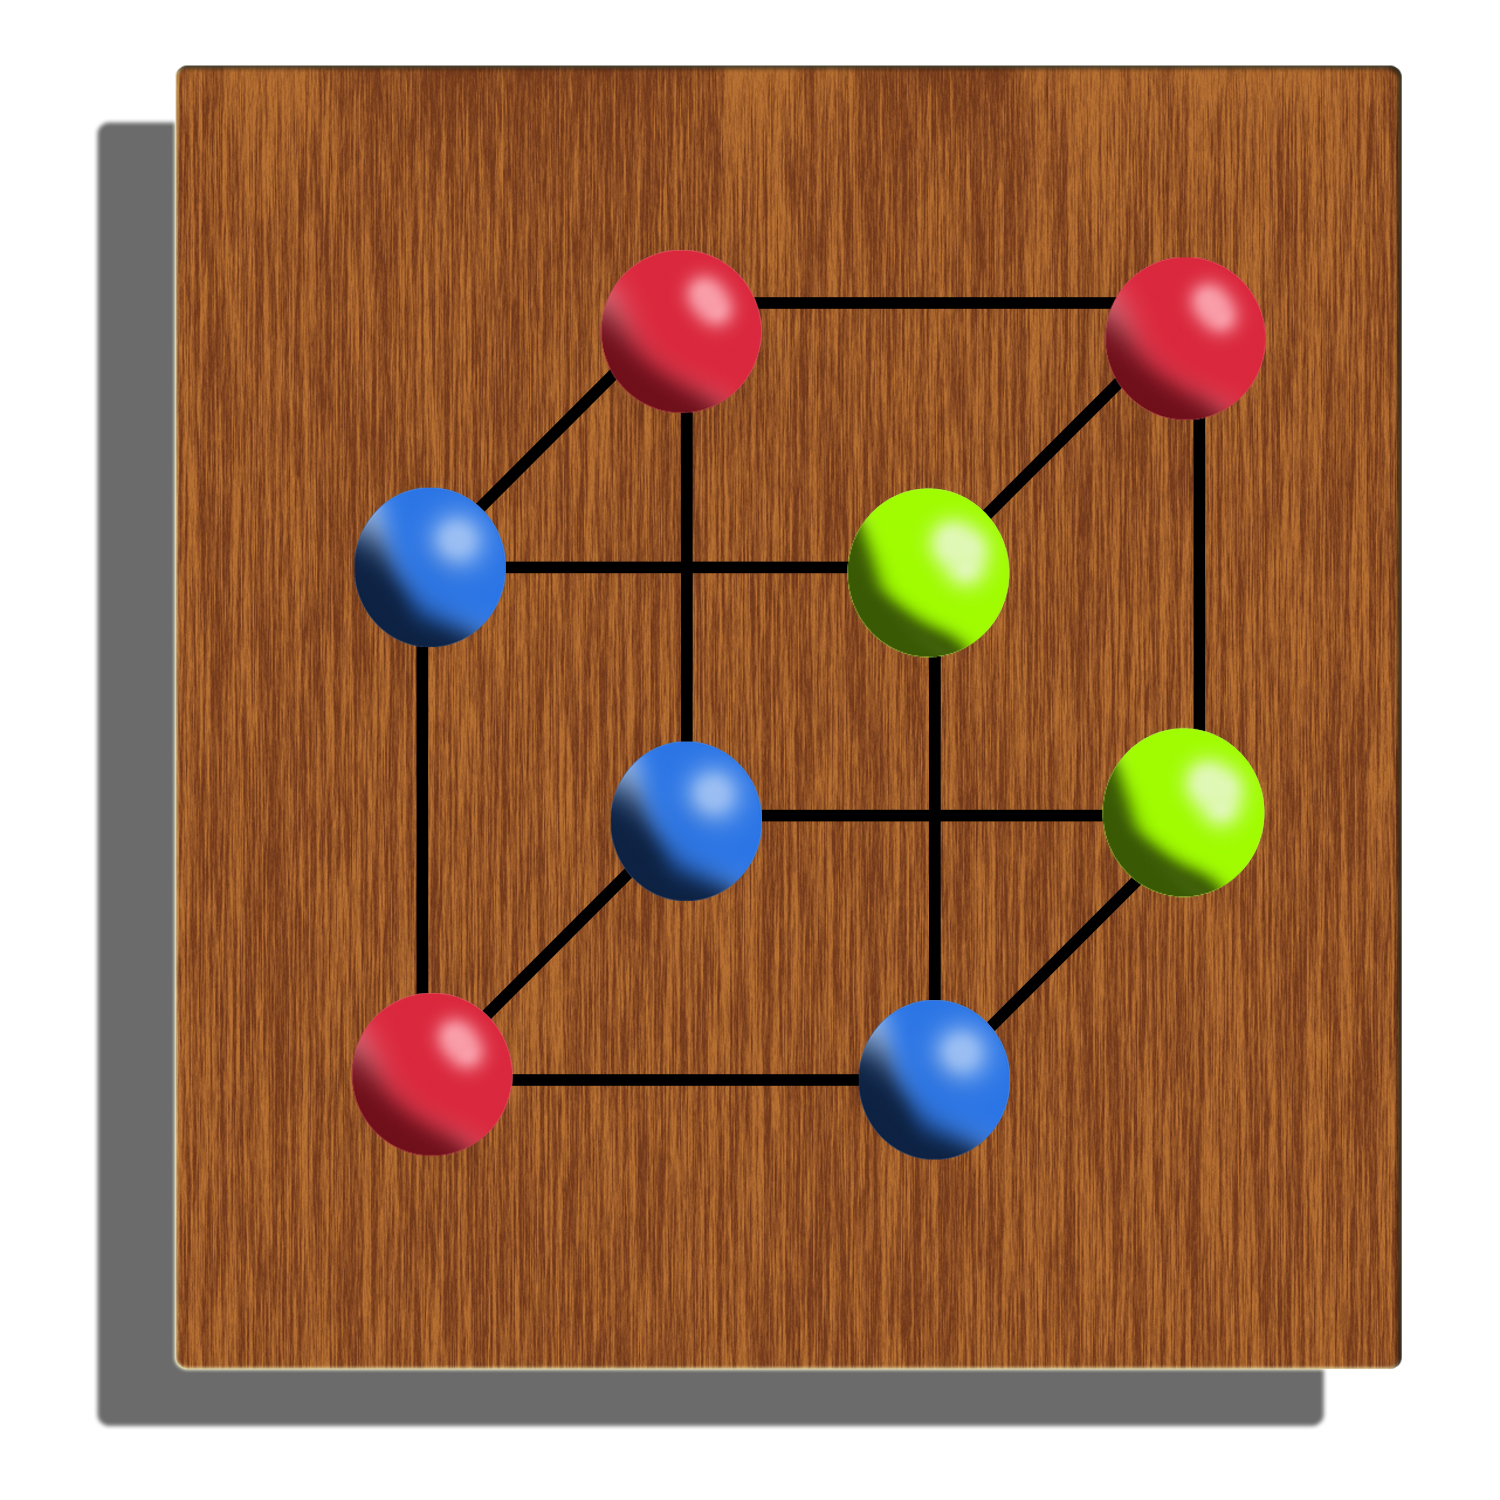
\includegraphics[width=400 px,height=400 px]{icon}
\caption{Icon}
\end{figure}

\newpage \ \newpage

\end{document}